\documentclass[12pt,a4paper]{article} 
\author{Abdelmalek Fathi, Maamar Choukri\\
Laarbi Tebessi Tebessa University\\
Math and Computer Science Departement}
\title{Build a web site for representing international conferences}
\date{}
\usepackage[left=12mm, top=1in, bottom=1.5in]{geometry}
\usepackage{graphicx}
\graphicspath{ {./images/} }
\renewcommand*\contentsname{Table of Contents}

\begin{document}
	\maketitle
	\clearpage
	\listoffigures
	\listoftables
	\clearpage
	\tableofcontents
	\clearpage
	\section{Introduction}
	\paragraph{}
	National and international scientific conferences are an important event for universities and researchers from different parts of the world, so it is necessary to facilitate the process of publishing and accessing these conferences.
	\subsection{Problematic}
	\paragraph{}
	Most or all universities of the world are publishing their conferences in custom web pages for each one, or they collect them in one website like 10times.com and ieee.org. Meanwhile any scholar how want to publish his paper or submit in a conference, he utilize another different website like easychair.org. Our work is related to finding a solution to the problem raised by answering the following questions:
	\begin{itemize}
		\item Why not they all publish everything from conferences to papers in one place ?
		\item How to let scholars and universities contact with each other from one place ?
		\item What is the best solution for this problem and how to achieve that ?
	\end{itemize}
	\subsection{Hypotheses}
	\paragraph{}
	Among the proposed solutions, we find that one of them relies on creating a website for publishing conferences and requesting registration in them, where the person in charge of the conference (university or organization) publishes the necessary information about the conference such as its name, date, and participation price, if any, while any researcher or student can Knowing the request to participate in it, as he sends his research to the officials in charge of the conference and is waiting for it to be accepted by them.
	\subsection{Article structure}
	\paragraph{}
	This article contains the following chapters:
	\begin{itemize}
		
		\item \textbf{Presentation of the project frameworks :}
		Chapter to figure out the problem and its solution in details.
		
		\item \textbf{Analysis and design \textit{(UML)} :}
		Chapter to introduce the \textit{UML} diagrams that we used to analysis the project and figure out his functions.
		
		\item \textbf{The implementation :}
		Chapter to view  the technologies that we used in making the site, and the implementation of our site (pictures from the website itself).
		
	\end{itemize}
	\clearpage
	\section{Presentation of the project frameworks}
	
	\clearpage
	\section{Analysis and design (UML)}
	We have utilized the following graphs: class, use cases and sequence diagram of each process in our website.
	
	\subsection{Class Diagram}
	a diagram to introduce classes of the project and their associations with each others.
	
		\begin{figure}[!h]
			\centering
			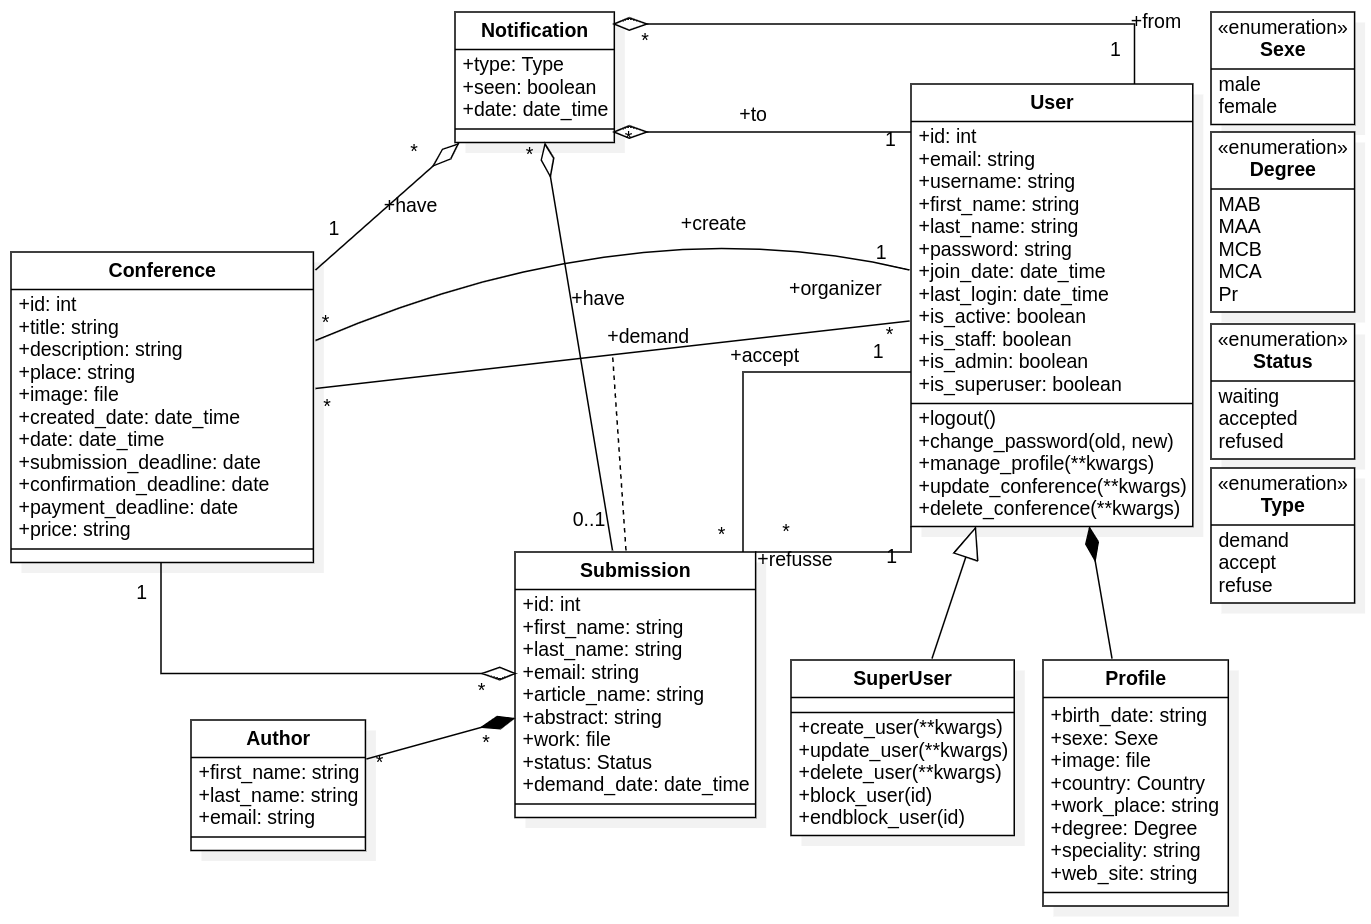
\includegraphics[width=\textwidth]{diagrams/class.png}
			\caption{class diagram}
			\label{fig:class-d}
		\end{figure}

	\subsection{Use case Diagram}
	a diagram to introduce what can every actor do in this project.
	
		\begin{figure}[!h]
			\centering
			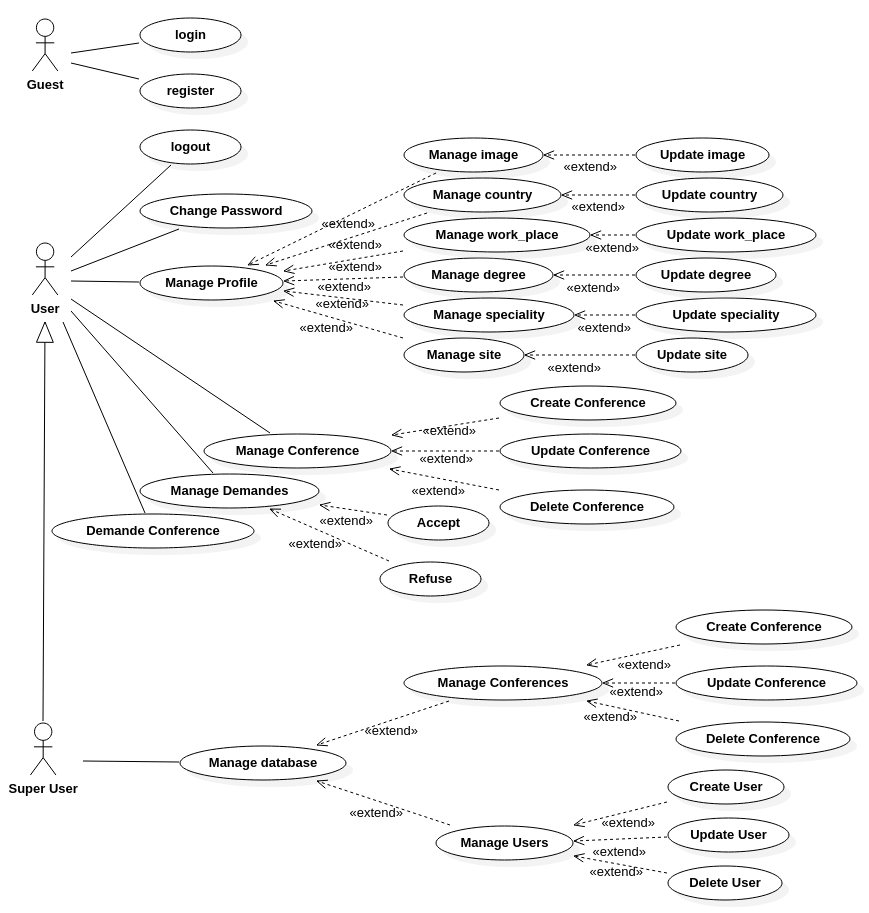
\includegraphics[width=\textwidth]{diagrams/use_case.png}
			\caption{use case diagram}
			\label{fig:use-case-d}
		\end{figure}

	\subsection{Sequence Diagrams}
	diagrams to figure out how each process is working behind the scene.
		\subsubsection{For add user}
		how to add new user
		
			\begin{figure}[!h]
				\centering
				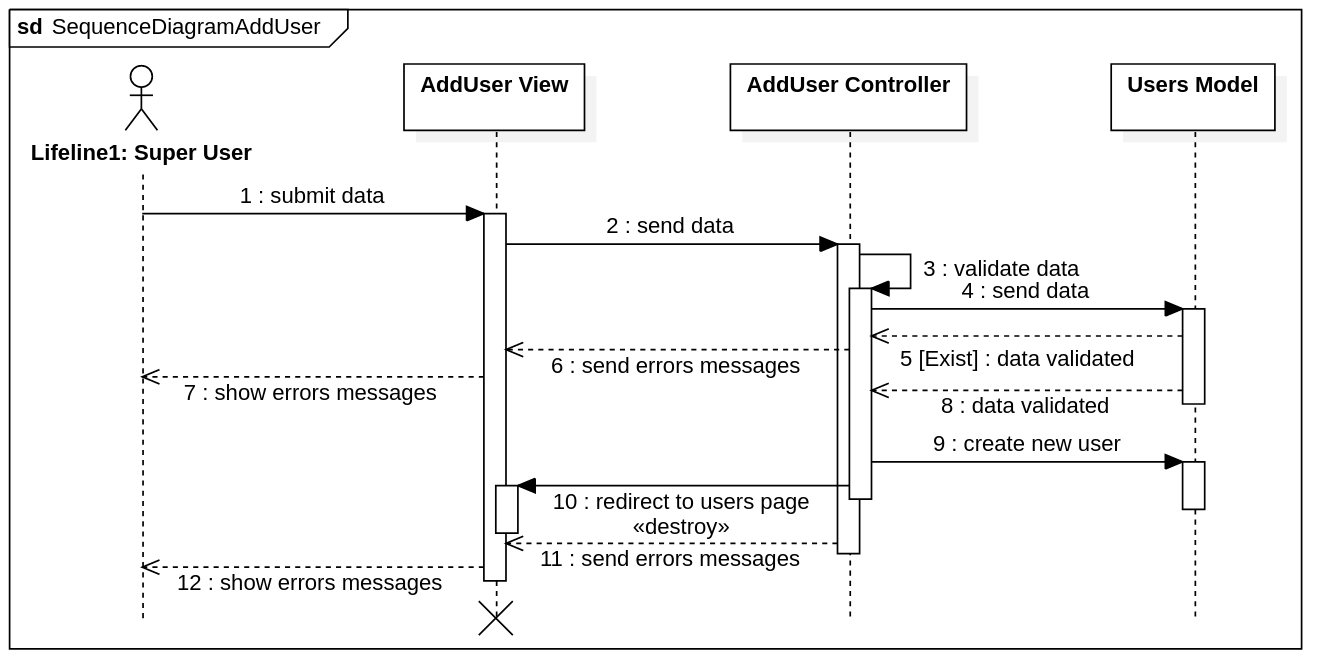
\includegraphics[width=\textwidth]{diagrams/add_user_sequence.png}
				\caption{add user sequence diagram}
				\label{fig:add-user-s-d}
			\end{figure}
		
		\subsubsection{For update user}
		how to update user information
		
			\begin{figure}[!h]
				\centering
				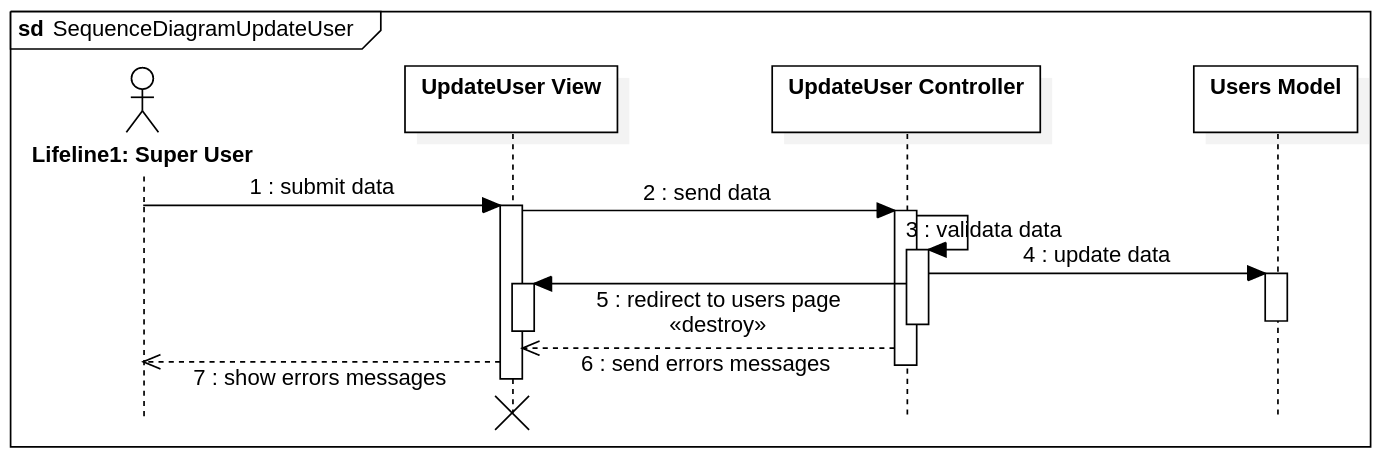
\includegraphics[width=\textwidth]{diagrams/update_user_sequence.png}
				\caption{update user sequence diagram}
				\label{fig:update-user-s-d}
			\end{figure}
		
		\subsubsection{For delete user}
		how to delete a user from the data base
		
			\begin{figure}[!h]
				\centering
				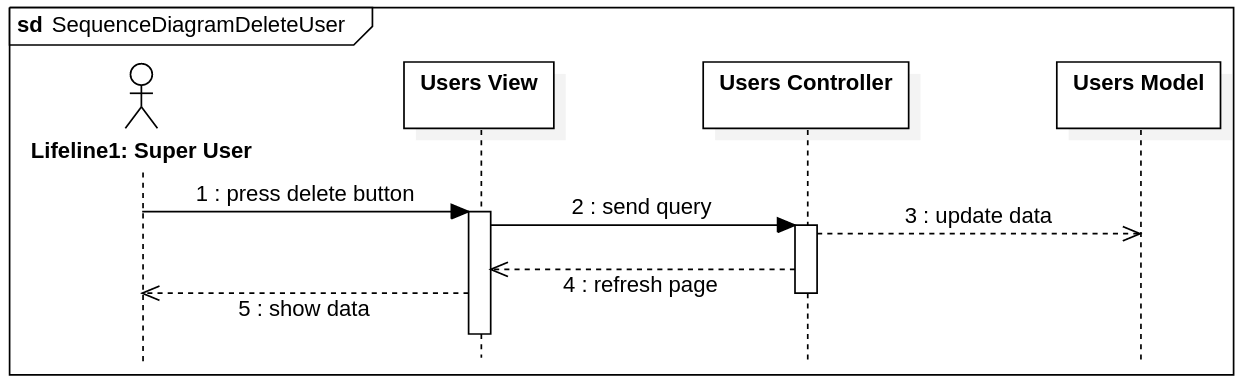
\includegraphics[width=\textwidth]{diagrams/delete_user_sequence.png}
				\caption{delete sequence diagram}
				\label{fig:delete-user-s-d}
			\end{figure}
		
		\subsubsection{For register}
		how to register as a new user
		
			\begin{figure}[!h]
				\centering
				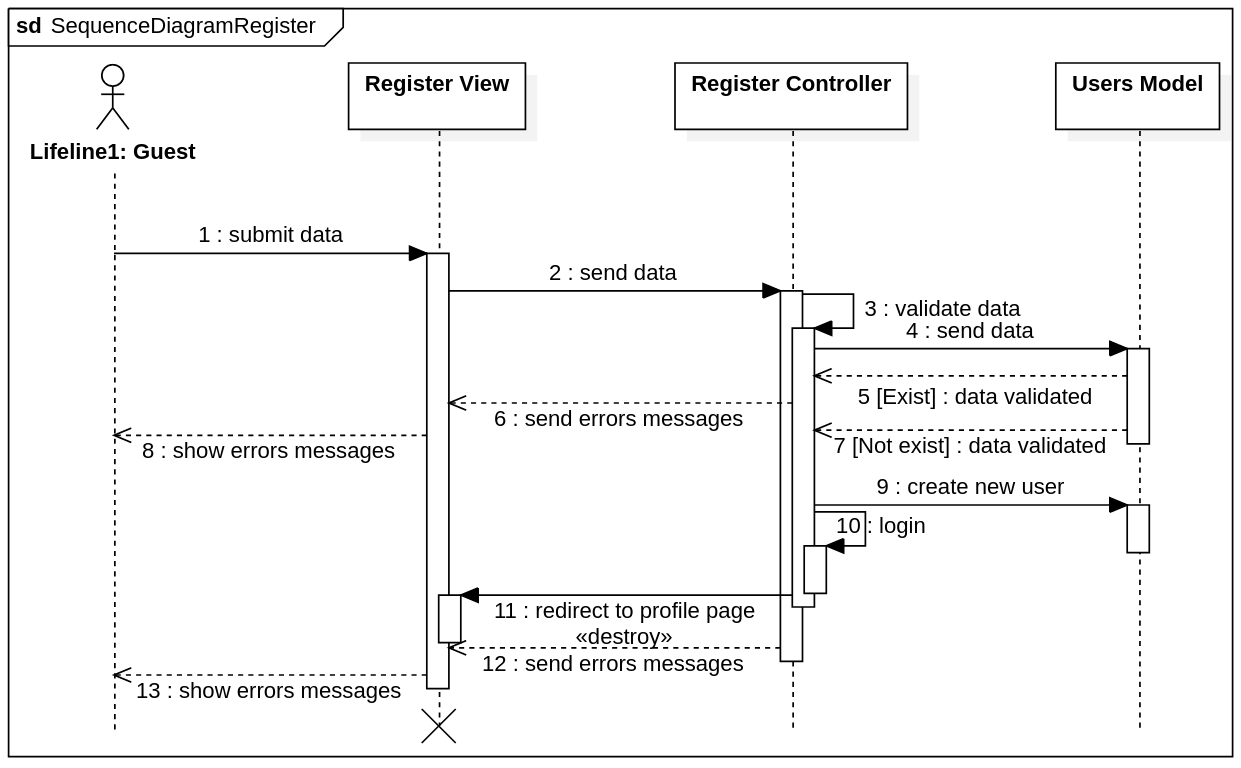
\includegraphics[width=\textwidth]{diagrams/register_sequence.png}
				\caption{register sequence diagram}
				\label{fig:register-s-d}
			\end{figure}
		
		\subsubsection{For login}
		how the user can login
		
			\begin{figure}[!h]
				\centering
				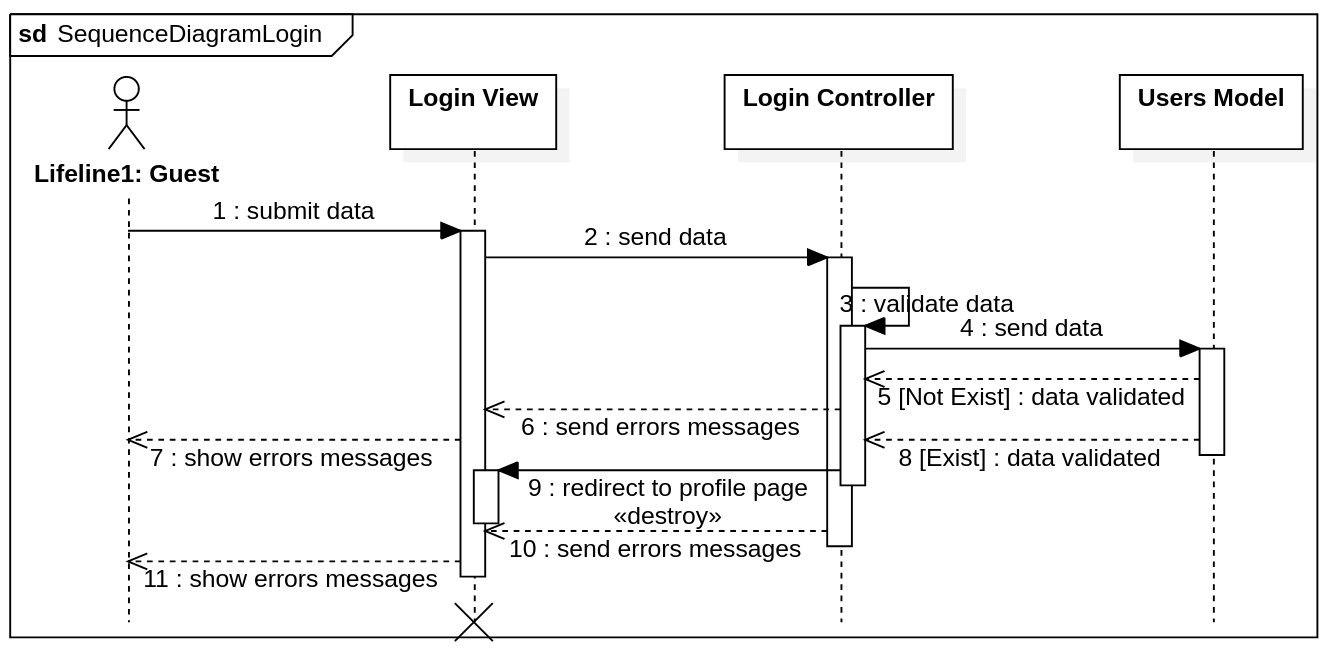
\includegraphics[width=\textwidth]{diagrams/login_sequence.png}
				\caption{login sequence diagram}
				\label{fig:login-s-d}
			\end{figure}
	
	\clearpage
	\section{The implementation}
	\paragraph{}
	There are many technologies that allow building web applications, and they are divided into two main parts, the front-end part such as HTML, CSS ..., and the back-end part such as PHP, NodeJS ..., in addition to databases, but we will depend in our project on the following:
	\subsection{Implementation Technologies}
	\subsubsection{For front-end}
	\paragraph{HTML}
	HTML (Hyper-Text Markup Language) is the standard mark-up language for documents designed to be displayed in a web browser. It can be assisted by technologies such as Cascading Style Sheets (CSS) and scripting languages such as JavaScript.\cite{HTML}
	\paragraph{CSS}
	Cascading Style Sheets (CSS) is a simple mechanism for adding style (e.g., fonts, colors, spacing) to Web documents.\cite{CSS}
	\subsection{For back-end}
	\subsubsection{For back-end}
	\paragraph{Django Web Framework}
	Django is a high-level Python Web framework that encourages rapid development and clean, pragmatic design. Built by experienced developers, it takes care of much of the hassle of Web development, so you can focus on writing your app without needing to reinvent the wheel. It’s free and open source.\cite{Django}
	\paragraph{why django ?}
	\begin{itemize}
		\item It's a Python Language.
		\item Built-in administration interface.
		\item Framework able to customization.
		\item large community.
		\item MVC design pattern.
		\item Built-in ORM for databases.
		\item Secured.
		\item and much more ...
	\end{itemize}
	\subsubsection{For databases}
	\paragraph{PostgreSQL}
	PostgreSQL is a powerful, open source object-relational database system with over 30 years of active development that has earned it a strong reputation for reliability, feature robustness, and performance.\cite{PostgreSQL}
	\clearpage
	\section{Conclusion}
	
	\clearpage
	\begin{thebibliography}{9}
		\bibitem{HTML}
		https://en.wikipedia.org/wiki/HTML
		\bibitem{CSS}
		https://www.w3.org/Style/CSS/Overview.en.html
		\bibitem{Django}
		https://www.djangoproject.com/
		\bibitem{PostgreSQL}
		https://www.postgresql.org/
	\end{thebibliography}
	
\end{document}
